\documentclass[conference]{IEEEtran}
\usepackage{graphicx, subfigure, algorithmic, algorithm, placeins, balance, color}
\usepackage{epstopdf}

\begin{document}

\title{Crowd-Shared Wireless Mesh Networks}

\author{
\begin{tabular}{cccc}
\multicolumn{1}{c}{Ahmed Abujoda$^{\dagger}$} &
\multicolumn{1}{c}{Arjuna Sathiaseelan$^{\S}$} &
\multicolumn{1}{c}{Panagiotis Papadimitriou$^{\dagger}$} &
\multicolumn{1}{c}{Jon Crowcroft$^{\S}$} \\ 
\end{tabular}\\
\\
$^{\dagger}$Institute of Communications Technology, Leibniz Universit\"at Hannover, Germany\\
\textit{\footnotesize{\{ahmed.abujoda, panagiotis.papadimitriou\}@ikt.uni-hannover.de}}\\
$^{\S}$Computer Laboratory, University of Cambridge, UK\\
\textit{\footnotesize{\{arjuna.sathiaseelan, jon.crowcroft\}@cl.cam.ac.uk}} \\
}

\maketitle

\begin{abstract}
Universal access to Internet is crucial, and as such, there have been several initiatives to enable wider access to the Internet. Public Access WiFi Service (PAWS) is one such initiative that takes advantage of the the available unused capacity in home broadband connections and allows Less-than-Best Effort (LBE) access to these resources, as exemplified by Lowest Cost Denominator Networking (LCDNet). PAWS has been recently deployed in a deprived community in Nottingham, and, as any crowd-shared network, it faces limited coverage, since there is single point of Internet access per guest user, whose availability depends on user sharing policies.

To mitigate this problem and extend the coverage, we consider a crowd-shared wireless mesh network (WMN) in which the home routers are interconnected as a mesh. Such a network provides multiple points of Internet access and can enable resource pooling across all available paths to the Internet backhaul. In this paper, we investigate the potential benefits of a crowd-shared WMN for public Internet access by performing a comparative study between such a network and PAWS, using simulations. To this end, we present an algorithm that selects the gateway and the shortest path for guest user traffic redirection through the WMN. Our simulations are driven from real user sharing patterns, collected from the PAWS deployment in Nottingham. Our simulation results show that a crowd-shared WMN can provide much higher utilization of the shared bandwidth and can accommodate a substantially larger volume of guest user traffic. We further investigate the trade-off between shared bandwidth utilization and the maximum number of hops between the local home router and the gateway.


\end{abstract}

\section{Introduction}

%The Internet has crossed new frontiers with access to it getting faster and cheaper. New applications and services are being offered. Information and communication is of utmost importance during emergency response. The Internet plays a crucial role in enabling access to critical information that can save lives of people. Internet is now seen as critical infrastructure � enabling remote health care, education, employment, e-governance, digital economy, and social networks. 

%In the reality of today�s Internet, the vision of digital inclusion faces the challenge of a growing digital divide, i.e., a growing disparity between those with sufficient access to the Internet and those who cannot afford the access to universal services. 

The Internet has evolved into a critical infrastructure for education, employment, e-governance, remote health care, digital economy, and social media. However, Internet today is facing the challenge of a growing digital divide, i.e., an increasing disparity between those with and without Internet access. Access problems often stem from sparsely spread populations living in physically remote locations, since it is simply not cost-effective for Internet Service Providers (ISPs) to deploy the required infrastructure for broadband Internet access in these areas. Coupled with physical limitations of terrestrial infrastructures (mainly due to distance) to provide last mile access, remote communities also incur higher costs for connection between the exchange and backbone network when using wired technologies, because the distances are longer. A large exchange may accommodate many users and allow for competition between service operators; in contrast, a rural/remote broadband connection does not usually offer economies of scale, increasing the costs per user. 

This problem is widely and publicly recognized. For example, in 2012 9.1 million homes in Europe still did not have fixed broadband coverage, more than 90\% of which are in rural areas \cite{BROAD2012}. Achieving ubiquitous mobile broadband coverage is also currently seen as not feasible by major operators as direct investment in local infrastructure may be uneconomic.

Addressing digital exclusion due to socio-economic barriers is also important. The United Nations revealed the global disparity in fixed broadband access, showing that access to fixed broadband in some countries costs almost 40 times their national average income \cite{FILD2010}. This problem is also applicable to developed countries where many individuals find themselves unable to pass a necessary credit check or living in circumstances that are too unstable to commit to lengthy broadband contracts \cite{LCDNet}. A recent survey in Nottingham, UK \cite{NCC2012} revealed that affordability is cited as the primary barrier, explicitly so by over 22.7\% of digitally excluded in the age of 16-44 years. 

We see enabling benevolence in the Internet (act of sharing resources) as a potential solution to solve the problem of digital exclusion caused due to socio-economic barriers. Lowest Cost Denominator Networking (LCDNet) \cite{LCDNet} is a new Internet paradigm that architects multi-layer resource pooling Internet technologies to support new low-cost access methods that could greatly reduce a network operator's direct investment in local infrastructure to support wider Internet access. LCDNet proposes to bring together several existing resource pooling Internet technologies to ensure that donors (users and network operators), who share their resources, are not affected and at the same time are incentivized for sharing their resources.  

Public Access WiFi Service (PAWS) \cite{PAWS} is based on LCDNet using a set of techniques that make use of the available unused capacity in home broadband networks and allowing Less-than-Best Effort (LBE) access to these resources \cite{LCDNet}. PAWS adopts an approach of community-wide participation, where broadband customers are enabled to donate controlled but free use of their high-speed broadband Internet by fellow citizens. Other initiatives have already explored sharing a user's broadband Internet connection via wireless (e.g., FON \cite{FON}). Although these methods are gaining worldwide acceptance, they are usually viewed as an extension of a user's paid service which is accessible only by other customers of the same service. In contrast, PAWS offers free access to essential services to all. 

To protect the consumer's paid service and the service provider revenue, it is essential to ensure that the guest user traffic does not impact perceived performance of the bandwidth donor (customer). The PAWS service is therefore constrained to offer a LBE access to network resources (lower quality compared to the standard Internet service offered to paying users). Various methods are being considered, including enabling LBE QoS (both in layers 2 and 3) in the network.

\begin{figure}[b]
\begin{center}
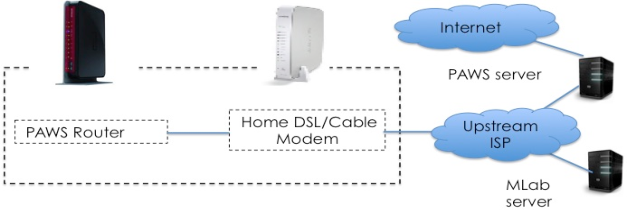
\includegraphics[width=1\linewidth]{paws.pdf}  
\caption{PAWS network.}
\label{fig:paws}
\end{center}
\end{figure}

PAWS is currently under deployment with 20 custom-made PAWS routers placed in a deprived community in Nottingham and another 10 routers in rural Scotland (Fig. \ref{fig:paws}). PAWS currently serves as a medium-scale open network measurement observatory in the UK allowing researchers to gather data about network availability, reachability, topology, security, and broadband performance from distributed vantage points in socio-economically deprived urban and rural areas. The PAWS deployment is essentially a crowd-shared access network (similar to FON) for under-privileged users in urban and rural communities. This provides the research community with a wealth of information on the needs of under-privileged users in terms of their access patterns and what do they use Internet access for. %The testbed also provides researchers the opportunity to understand behavioral patterns of home broadband users in terms of how do they share their home broadband networks with the public, e.g., how often do they switch off their home access points and when (day/time) do they switch it off. 
However, PAWS has faced ongoing deployment challenges, such as limited coverage, due to home user sharing patterns (i.e., home network users stop sharing their Internet connection for certain periods).

In this paper, we investigate the potential benefits of enabling PAWS or any crowd-shared wireless network as a crowd-shared wireless mesh network (WMN). Leveraging on the principles of software-defined networks (SDN), we perform a comparative study between PAWS and a crowd-shared WMN, considering the WMN managed by a centralized SDN controller with a global network view. To this end, we generate a model for home network user sharing patterns based on the router on/off periods captured from the PAWS deployment. Using simulations, we show that a crowd-shared WMN can achieve very high utilization of the shared bandwidth and can accommodate a significantly larger volume of guest user traffic compared to PAWS.

The remainder of the paper is organized as follows. In Section \ref{sec:architecture}, we discuss the management of the WMN and present techniques for guest user traffic redirection. In Section \ref{sec:evaluation}, we present our simulation environment and discuss the benefits of using a crowd-shared WMN for public Internet access. Finally, Section \ref{sec:conclusion} highlights our conclusions.

\section{Crowd-Shared Wireless Mesh Networks}
\label{sec:architecture}

\begin{figure}[t]
\begin{center}
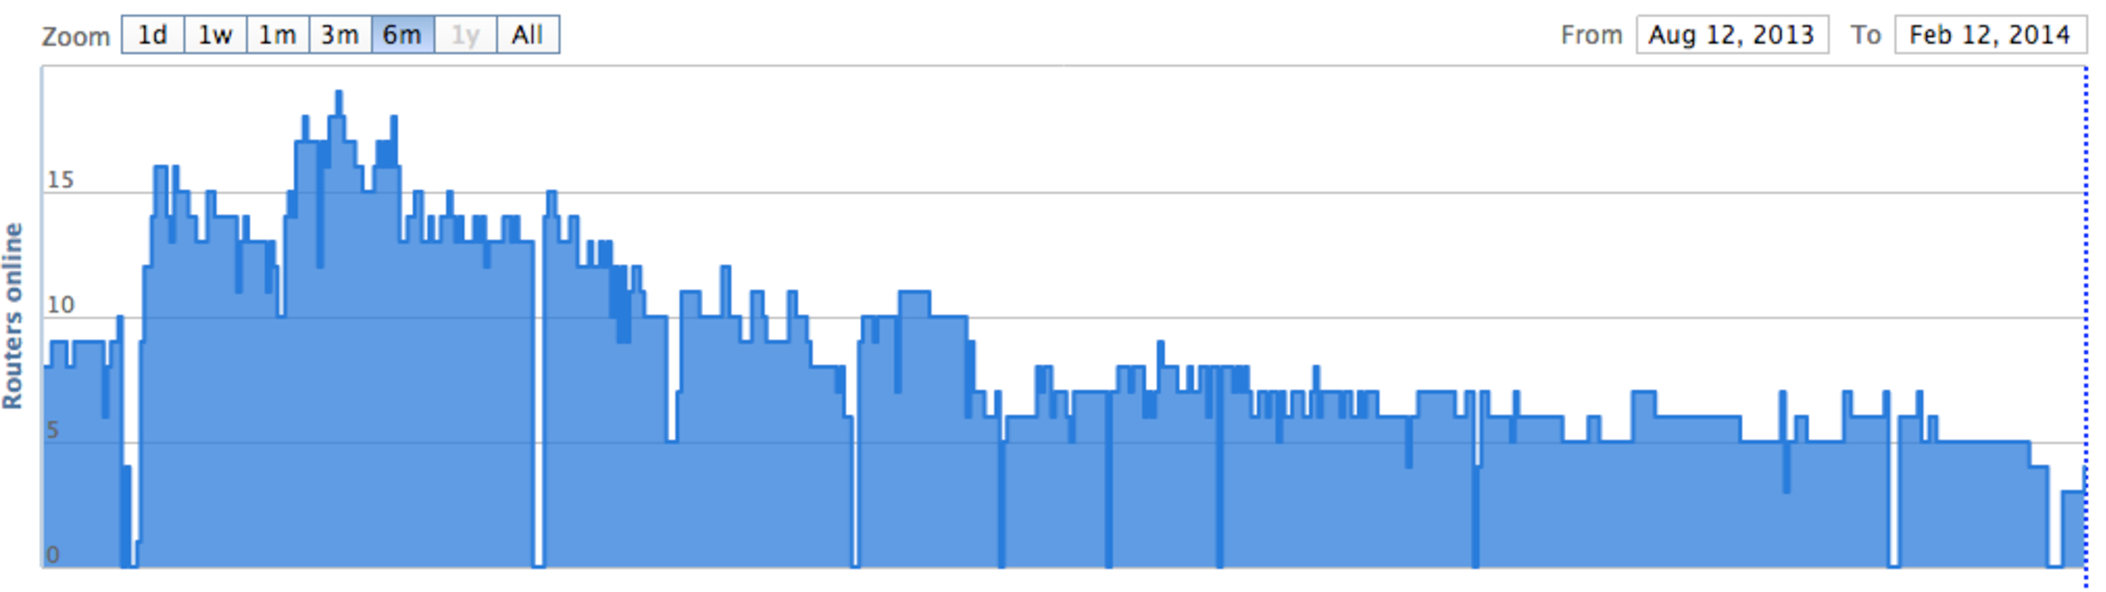
\includegraphics[width=1\linewidth]{paws-avail.pdf}  
\caption{PAWS routers availability.}
\label{fig:paws-avail}
\end{center}
\end{figure}

The underlying problem with PAWS or any crowd-shared network is that they serve as single point of Internet access to guest users within the coverage of the wireless router and hence, they have no provision to extend the coverage when no bandwidth is being shared. Based on our experience from the trial PAWS deployment, PAWS routers were not available for certain periods, because sharers needed all the bandwidth of their broadband connection or due to other reasons, such as economic constraints placed on home users in underprivileged areas where they are forced to conserve energy by turning off the routers at nights. In this respect, Fig. \ref{fig:paws-avail} illustrates a six-month view of the PAWS routers status (available/unavailable) logs demonstrating that not a single router was available continuously over the entire duration. These observed user behaviors entail significant challenges for the successful adoption of PAWS. 

\subsection{Crowd-Shared WMN Management}
\label{architecture:management}

A potential solution to this problem is to extend the PAWS network as a crowd-shared WMN. Such a network would allow home network users to share part of their own broadband connection to the public for free while also connected to each other as a WMN providing extended coverage (Fig. \ref{fig:wmn}). Extending PAWS to a crowd-shared WMN departs from the norm: multiple users from different ISPs form part of the WMN to provide free Internet connectivity, while most wireless community WMNs today are operated by a single organization. This raises important questions regarding the operation, configuration, and management of crowd-shared WMNs.  

\begin{figure}[t]
\begin{center}
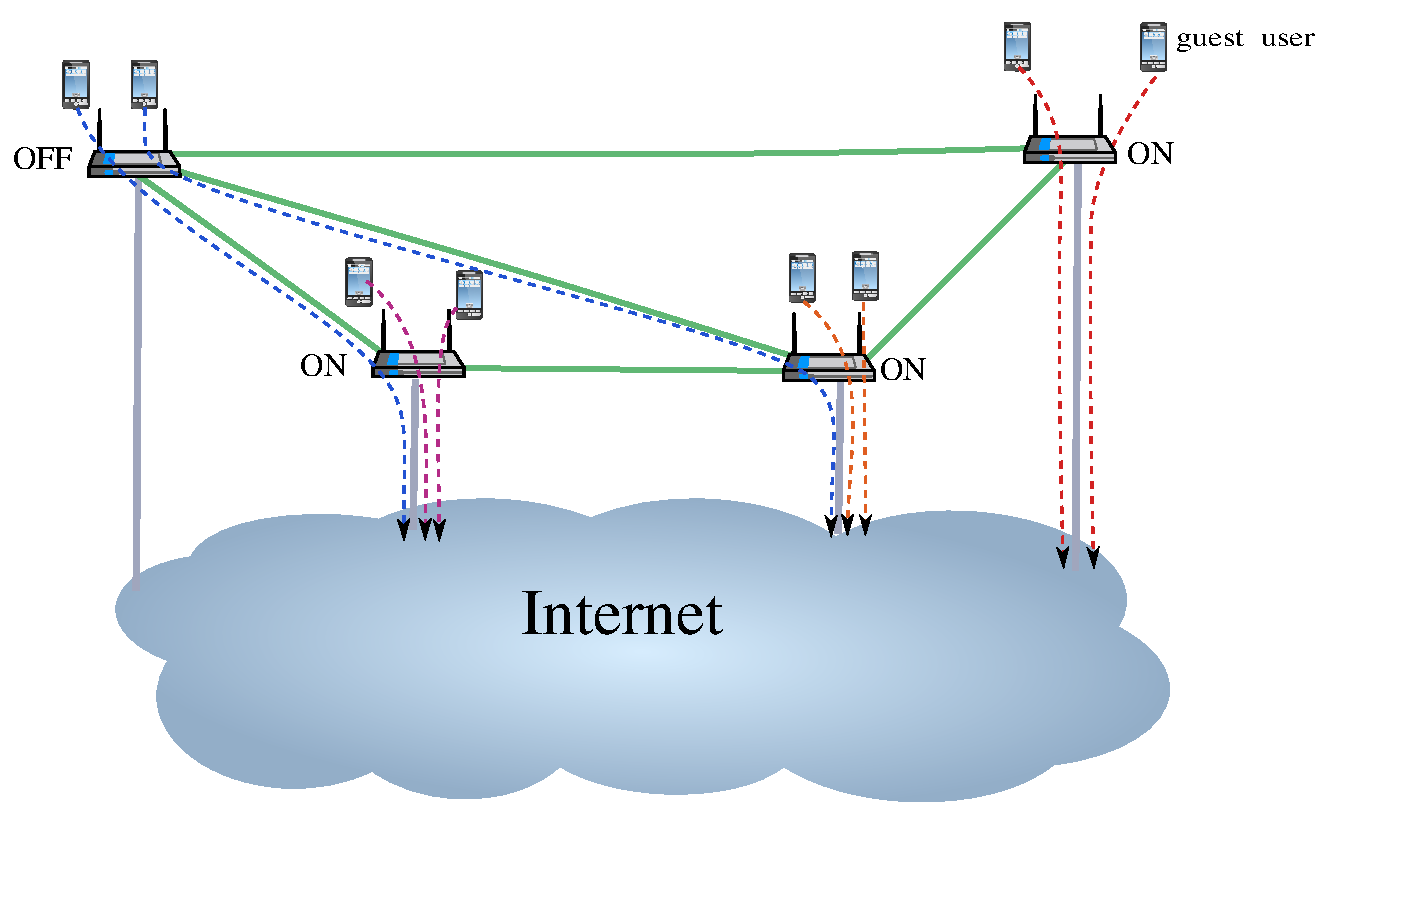
\includegraphics[width=1\linewidth]{flow_redirection.pdf}  
\caption{Crowd-shared WMN for public Internet access.}
\label{fig:wmn}
\end{center}
\end{figure}

SDN can facilitate the management and operation of wireless networks at large scale. Leveraging on SDN's centralized control and network-wide visibility, the management and operation of a crowd-shared WMN can be outsourced to a third party. In \cite{EWSDN}, we describe a holistic approach of coupling both social and economic incentives in designing future networks allowing the extension of the stakeholder value chain to include more than the two traditional parties (consumer and Internet service provider). Such an approach would provide opportunities for non-governmental organizations and local governments (driven by social goals rather than economic) to become virtual network operators. Enabling a third party to federate such wireless home networks would reduce the operating expenditures for network operators as well as enable new economic models for revenue creation from currently underutilized infrastructures. In particular, we rely on SDN to create the notion of Virtual Public Networks (VPuN), i.e., crowd-shared home networks created, deployed and managed through an evolutionary SDN control abstraction \cite{EWSDN}. Although originally intended for crowd-shared wireless networks such as PAWS, VPuN can also facilitate management of crowd-shared WMNs, enabling resource pooling across multiple home broadband connections based on the prevailing network conditions and usage sharing patterns. The VPuN architecture allows home broadband users to explicitly express policies on how and when they want the network to be shared.

\subsection{Traffic Redirection}
\label{architecture:redirection}

To take advantage of the extended coverage provided by a WMN, we develop and evaluate techniques for the redirection of guest user traffic during the periods that the home user does not permit the sharing of his broadband connection. In this case, Internet is accessed through the router of another home network where sharing is allowed. 

In the following, we present an algorithm (Algorithm \ref{alg:assignment}) for the assignment of the gateway and the path over which the traffic will be redirected through the WMN. We assume that this algorithm will be executed by a SDN controller which has knowledge of the WMN topology and utilization as well as the broadband connection utilization and user sharing policies. 

We represent the WMN as a weighted undirected graph $G = (N, L)$, where $N$ is the set of nodes and $L$ is the set of links between nodes of the set $N$. Each node $n_i$ is associated with an Internet access link whose available shared bandwidth is denoted by $C(n_i)$. Each link $l_{ij} \in L$ between two nodes $n_i$ and $n_j$ is associated with the available bandwidth $C(l_{ij})$. Let $P_{ij}$ denote the set of paths in the network $G$, between the pair of nodes $n_i$ and $n_j$. The available bandwidth $C(p)$ associated to a path $p \in P_{ij}$ is given by the minimum residual bandwidth of the links along the path:

\begin{equation}
C(p) = \min_{l_{ij} \in p} C(l_{ij}))
\end{equation}

We further represent a flow demand for a guest user with the tuple $d = (n_u, r)$, where $n_u \in N$ is the node where the guest user device has been attached and $r$ denotes the flow rate. We use $D$ to represent the set of flow demands that have arrived in the system.

\algsetup{indent=0em}
\begin{algorithm}[htbp]
  \caption{Gateway and Path Assignment}
  \label{alg:assignment}
  \begin{algorithmic}
  \small
    \STATE \textbf{Inputs}: $G = (N, L), D$
    \vspace{2mm}
    \STATE  SORT($D$)
    \vspace{0.7mm}
    \FOR{each $d \in D$}
    \vspace{0.7mm}
    \STATE \hspace{0.4cm} $search \leftarrow$ true
    \vspace{0.7mm}
    \STATE \hspace{0.4cm} $M \leftarrow \{N \setminus {n_u}\}$ \hspace{0.3cm} // $M:$ candidate set of routers
    \vspace{0.7mm}
    \STATE \hspace{0.4cm} \textbf{while} ($search$ AND $M \neq \emptyset$)
    \vspace{0.7mm}
    \STATE \hspace{0.8cm} $g \leftarrow argmax_{i \in M} C(n_i)$
    \vspace{0.7mm} 
    \STATE \hspace{0.8cm} \textbf{for} each $p \in P_{ug}$
    \vspace{0.7mm}
    \STATE \hspace{1.2cm} \textbf{if} $C(p) < r$ \textbf{then}
    \vspace{0.7mm}
    \STATE \hspace{1.6cm} $P_{ug} \leftarrow P_{ug} \setminus {p}$
    \vspace{0.7mm}
    \STATE \hspace{1.2cm} \textbf{end if}
    \vspace{0.7mm}
    \STATE \hspace{0.8cm} \textbf{end for}
    \vspace{0.7mm}
    \STATE \hspace{0.8cm} \textbf{if} $P_{ug} = \emptyset$ \textbf{then}
    \vspace{0.7mm}
    \STATE \hspace{1.2cm} $M \leftarrow M \setminus {n_g}$
    \vspace{0.7mm}
    \STATE \hspace{0.8cm} \textbf{else}
    \vspace{0.7mm}
    \STATE \hspace{1.2cm} gateway $\leftarrow n_g$ \hspace{0.6cm} // gateway assignment
    \vspace{0.7mm}
    \STATE \hspace{1.2cm} $path \leftarrow \mathrm{SP} (P_{ug})$ \hspace{0.3cm} // path assignment
    \vspace{0.7mm}
    \STATE \hspace{1.2cm} $search \leftarrow$ false
    \vspace{0.7mm}
    \STATE \hspace{0.8cm} \textbf{end if}
    \vspace{0.7mm}
    \STATE \hspace{0.4cm} \textbf{end while}
    \vspace{0.7mm}
    \ENDFOR
  \end{algorithmic}
\end{algorithm}

The algorithm assigns a gateway and the shortest path to each flow demand from the set $D$. The algorithm is executed whenever there is insufficient shared bandwidth in the local home network. Initially the flow demands are sorted based on the flow rate in decreasing order. For each flow demand, the algorithm selects the home router with the highest bandwidth in its access link (i.e., $C(n_i)$). Subsequently, the algorithm identifies the set of paths between the local home router ($n_u$) and the assigned gateway ($n_g$) that satisfy the flow rate requirement (Equation 1). In case there is no such path, the algorithm performs another iteration for the selection of the gateway, excluding the previously selected home router. Otherwise, the shortest among these paths is being identified based on the number of hops (SP function in the algorithm). This eventually designates the path for the traffic redirection through the WMN.

This algorithm carries out the gateway assignment based on the available shared bandwidth of the home routers in the crowd-shared network. Although this can pool resources from all home networks where sharing is permitted achieving efficient utilization of the shared bandwidth, guest user traffic may have to traverse multiple hops in the WMN. This can lead to latency inflation, delay variation and in general, unpredictable performance. To mitigate this, we further use a variant of this algorithm by introducing a threshold in the number of hops between the local home router and the assigned gateway. For example, adjusting the threshold to 1 restricts the search space to the next-hop routers with sufficient shared bandwidth.



\section{Evaluation}
\label{sec:evaluation}

In this section, we quantify the benefits of using a crowd-shared WMN for public Internet access. In Section \ref{evaluation:environment}, we present the simulation environment, the modeling of router on/off periods, and the metrics used to evaluate the WMN efficiency. Section \ref{evaluation:results} provides a comparative study between a crowd-shared network, such as PAWS, and a WMN based on our simulation results.

\subsection{Simulation Environment}
\label{evaluation:environment}

%Using python, we developed a discrete event simulator to model the behavior of guest flows in a crowd-shared network connected through a wireless mesh network. We use the TFA wireless mesh topology \cite{}, that consist of 21 nodes to model a network of access home routers. Each router possesses an Internet connection from which it provides potential guests with a maximum of 8 Mbps in upload direction. In addition, the nodes are interconnected using an 802.11ac wireless mesh network with a capacity of 200 Mbps.

We developed a simulator that models the behaviour of data flows that are generated by guest users in a crowd-shared WMN. We use the TFA wireless mesh topology \cite{TFA} which consists of 21 nodes (Fig. \ref{fig:topology}). Each node in this figure represents a home router with shared Internet access bandwidth, whereas each edge is a wireless mesh link. Guest user flows arrive randomly at different home routers. Each generated flow has a rate and lifetime sampled out of a uniform and an exponential distribution, respectively. The guest user flows arrive to the network according to a Poisson process.

We model the availability of the home access routers using an on-off Markov chain. On and off times are exponentially distributed with mean values $\mu_{on = 106}$ minutes and $\mu_{off} = 555$ minutes. We parameterize the exponential distributions using real datasets from the PAWS deployment in UK. Fig. \ref{fig:active_routers} shows the number of active routers along 60 hours of simulation. We can see that out of 21 routers less than 12 routers are simultaneously available.

%To reflect real world traffic, we consider guest flows that arrive to the network according to a Poisson process. Each flow has a constant bit rate which is sampled out of a uniform distribution.

\begin{figure}[t]
\begin{center}
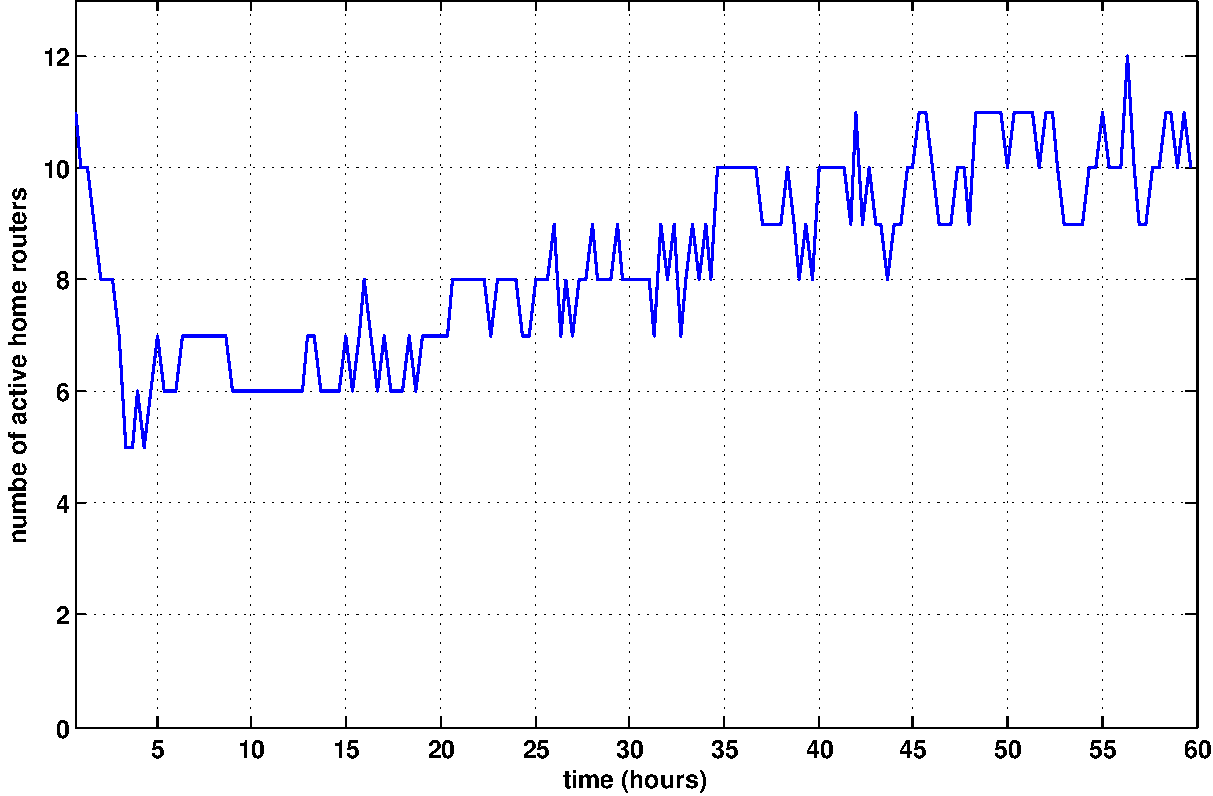
\includegraphics[width=1\linewidth]{results/on_routers.pdf}
\caption{Number of active home routers.}
\label{fig:active_routers}
\end{center}
\end{figure}

%To grant Internet access to the flows, the simulator implements two methods. The first method only give access to flows through the router at which they arrive given that there is enough internet access capacity. This method ignores the mesh network. On the other hand, the second method considers the mesh network by redirecting flows which does not fit in the local access routers to other routers through the mesh network. The router to which the flow is redirected are selected using worst-fit decreasing algorithm. The algorithm starts by sorting the flows to be redirected in non-decreasing order of their rates. Then, for each flow (starting with the flow with the highest rate), the algorithm selects the router with the highest available internet access capacity which fits the flow rate. The shortest path between the router is chosen based on the number of hops. The worst-fit decreasing algorithm is also used to redirect flows when a router goes OFF. This sustains as much as possible flows in the network and reduce disruption by the routers owners sharing policy.
%Furthermore, to show performance of the system under dynamic communication pattern, we consider flows with limited life time which arrive and leave the system at certain time point.

\begin{figure}[t]
\begin{center}
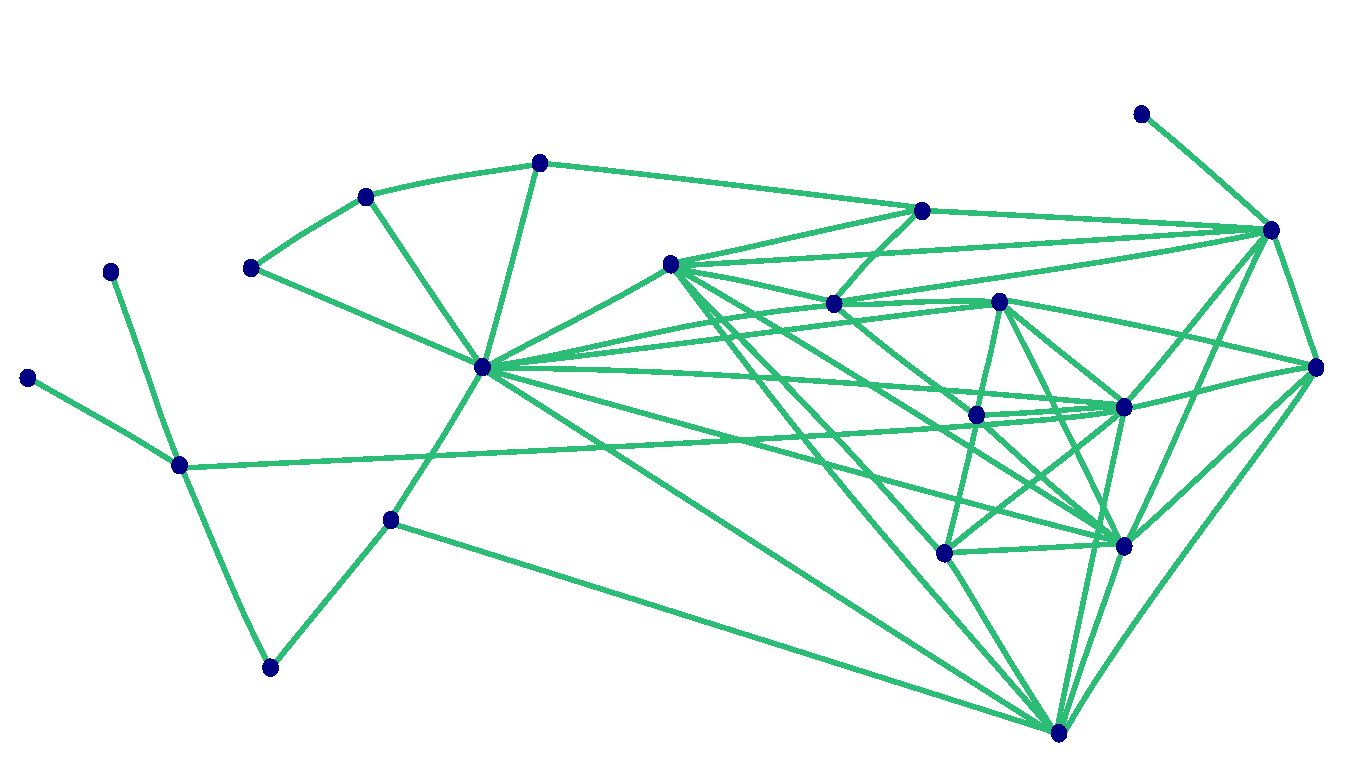
\includegraphics[width=1\linewidth]{topology.pdf}
\caption{Simulation WMN topology.}
\label{fig:topology}
\end{center}
\end{figure}

Guest user flows are granted Internet access either through local routers or by redirection to remote routers based on the algorithm presented in Section \ref{architecture:redirection}. Flows which cannot be accommodated are rejected. We evaluate the benefit of WMN in the context of crowd-shared Internet access using the total shared bandwidth utilization in all home routers as well as the accumulated acceptance rate. We define the accumulated acceptance rate $ACR(T)$ at time $T$ as:

\begin{equation}\label{1}
ACR(T)= \frac{\Sigma^T_t s^{finished}_{t}}{(\Sigma^T_t s^{finished}_{t} + \Sigma^T_t s^{rejected}_{t})},
\end{equation}
%
%${the accumulated acceptance rate =\displaystyle \frac{the\ total\ rates\ of\ flows\ finished\ up\ to\ t} {(the total rates of flows finished up to t + total rates of rejected flows up to t)}}$.
where $s^{finished}_{t}$ denotes the total flow sizes of the flows at time $t$ which are accepted (assigned Internet access) and successfully served without disruption due to router unavailability. $s^{rejected}_{t}$ denotes the total sizes of the flows at time $t$ which are rejected (not assigned Internet access).

Each simulation run comprises 60 hours at a time discretization of 20 minutes. For each scenario, we perform 20 simulation runs. We assume a homogeneous setting where each router has 16 Mbps ADSL downlink and set the shared bandwidth per router to 8 Mbps (i.e., over the periods that each router is active). We run our simulation with mesh link capacity of 200, 54 and 10 Mbps; this does not have any impact on the simulation results, since the bottleneck is the Internet access links. Our wireless link model does not consider the impact of interference and distance on the offered link bandwidth.

\subsection{Simulation Results}
\label{evaluation:results}

Initially, we measure the shared bandwidth utilization and acceptance rate with an arrival rate of 50 flows per minute over a 60-hour period. Fig. \ref{fig:utilization} illustrates a low utilization of the shared bandwidth without a WMN during the whole period, although there is high demand for Internet access by guest users attached to the various home networks. In contrast, a WMN allows to capitilize the unused capacity and accommodate a larger volume of guest user traffic. More precisely, according to Fig. \ref{fig:utilization} guest user traffic redirection through the WMN results in the full utilization of the shared bandwidth. Furthermore, crowd-shared WMNs can accommodate substantially larger volume of guest user traffic, as depicted in Fig. \ref{fig:acceptance}. This stems from the high utilization of the shared bandwidth.

\begin{figure}[t]
\begin{center}
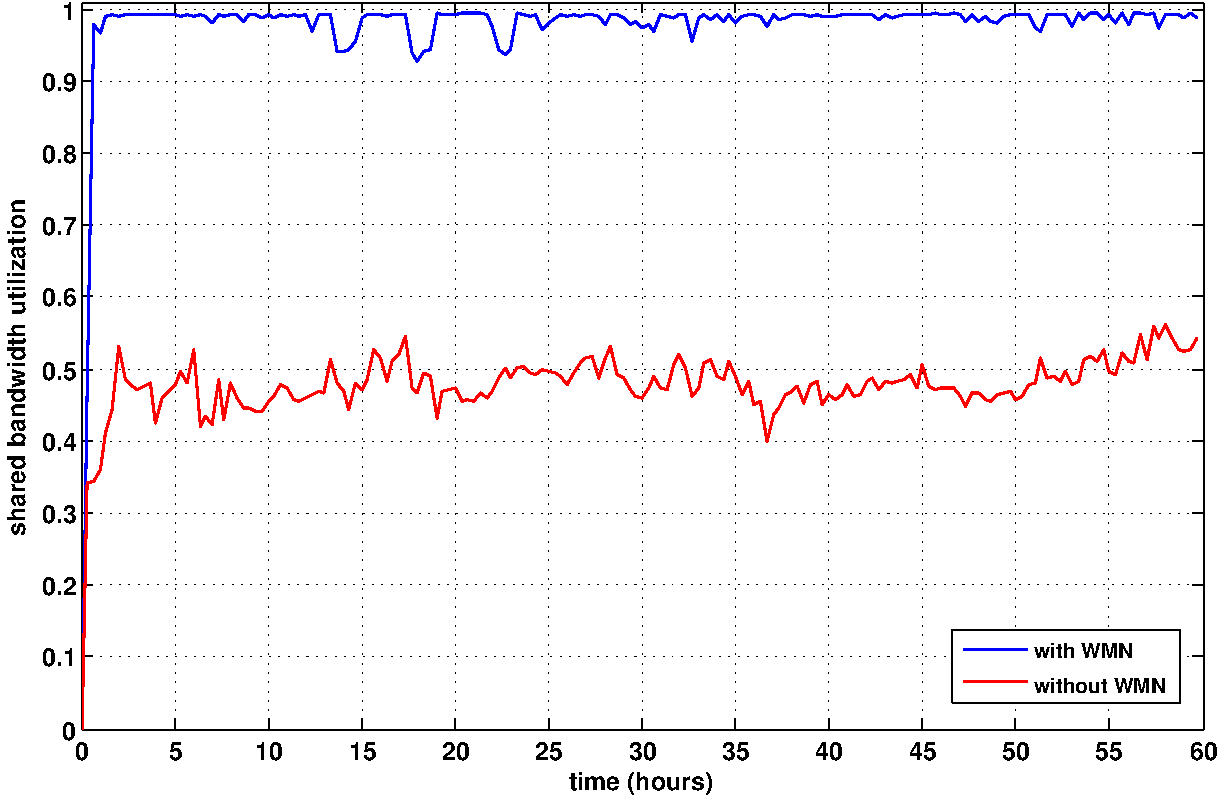
\includegraphics[width=1\linewidth]{results/utilization.pdf}
\caption{Shared bandwidth utilization.}
\label{fig:utilization}
\end{center}
\end{figure}

\begin{figure}[t]
\begin{center}
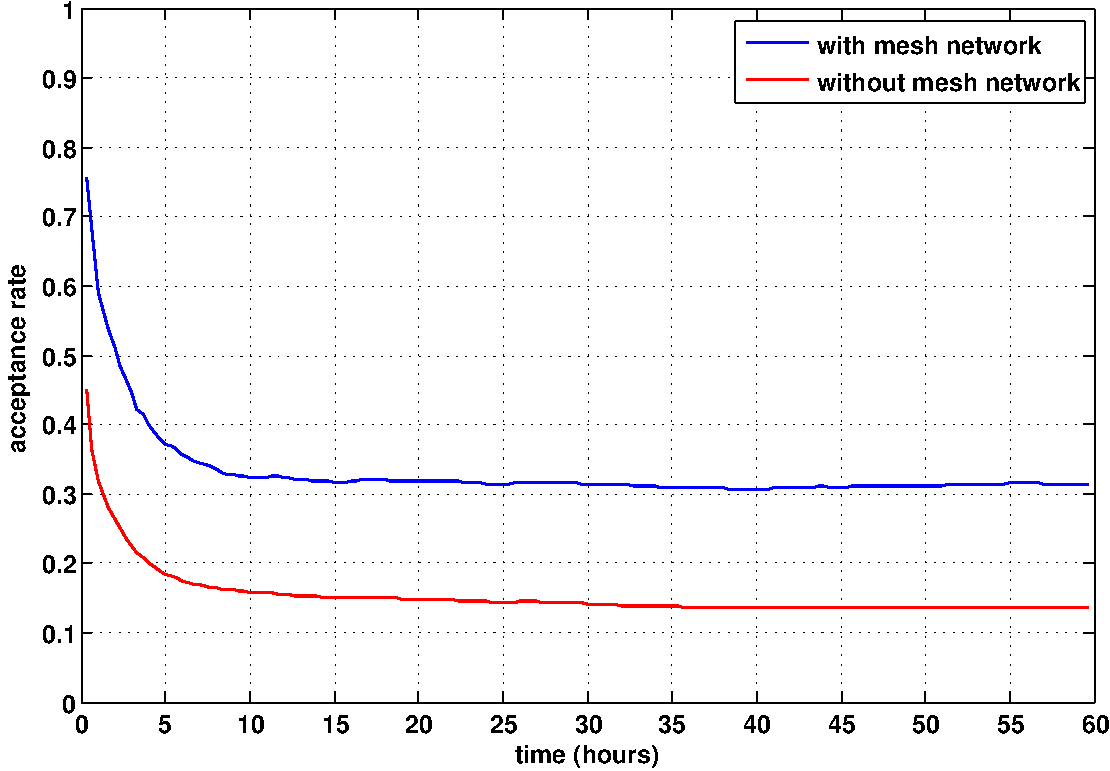
\includegraphics[width=1\linewidth]{results/acceptance_rate.pdf}
\caption{Guest user traffic acceptance rate.}
\label{fig:acceptance}
\end{center}
\end{figure}

We further measure the shared bandwidth utilization with a wide range of guest user traffic demands. In this respect, Fig. \ref{fig:acceptance} illustrates the shared bandwidth utilization with diverse flow arrival rates, ranging from 10 to 100 flows per minute. This simulation result corroborates the efficiency of the WMN for various traffic loads, as the shared bandwidth utilization always remains very high. Fig. \ref{fig:utilization_arrival} shows poor bandwidth utilization without a WMN, especially with low guest user traffic demand. In this particular case, the limitation of one point of Internet access for each guest user leads to wasting most of the shared bandwidth. Essentially, our simulation results show the significant benefit that a WMN can bring into crowd-shared networks, by effectively pooling resources across all home networks.

\begin{figure}[t]
\begin{center}
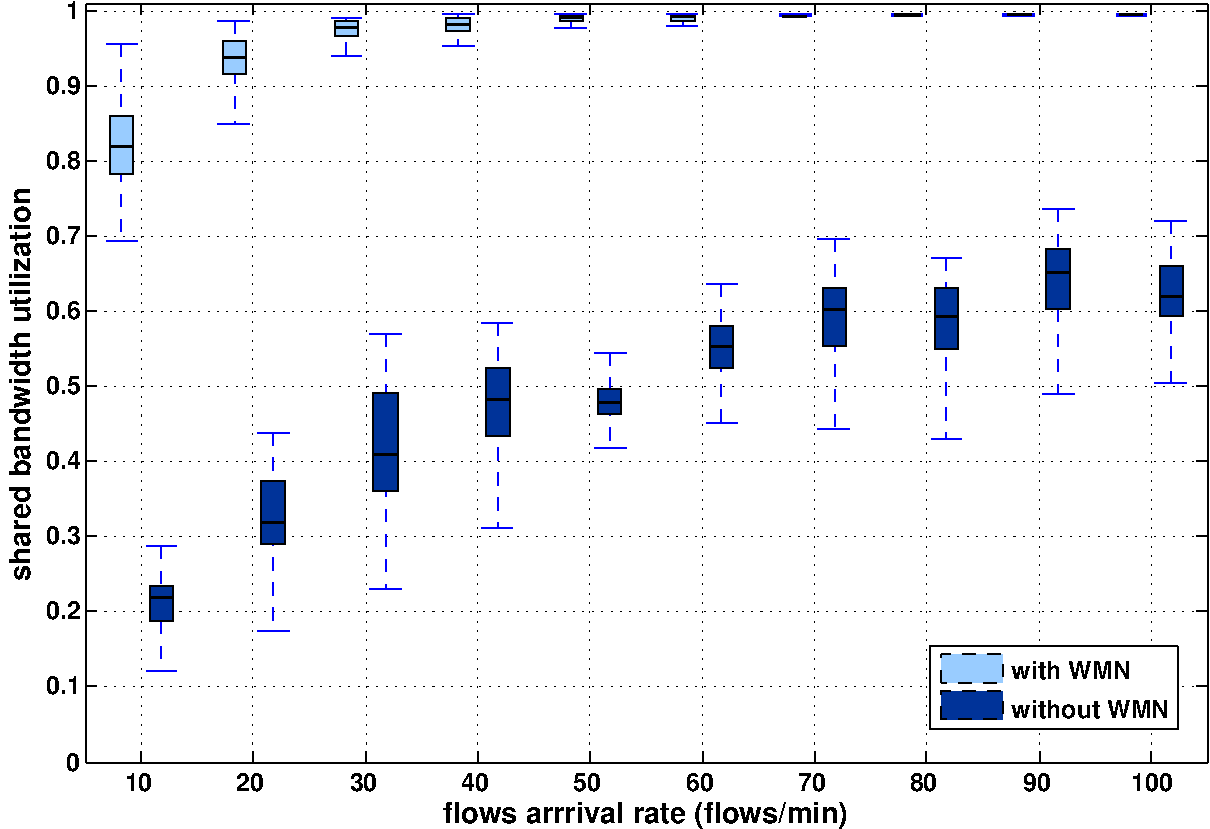
\includegraphics[width=1\linewidth]{results/boxplot2.pdf}
\caption{Shared bandwidth utilization vs. flow arrival rate.}
\label{fig:utilization_arrival}
\end{center}
\end{figure}

According to our simulations, redirected guest user traffic traverses up to 4 hops in the WMN. We further use a variant of our gateway and path assignment algorithm (briefly discussed in Section \ref{architecture:redirection}) which introduces a threshold in the number of hops between the home router and the assigned gateway. Fig. \ref{fig:hop_count} illustrates the shared bandwidth utilization for diverse hop-count threshold values ranging from 1 to 3, and without any limit in the hop count. Restricting the number of hops has a noticeable impact on bandwidth utilization, especially for a single hop, since Internet access is permitted only through one of the next-hop home routers. In essence, there is a trade-off between coverage extension (and thus effective bandwidth utilization) and latency. This may become more critical in large WMNs, where multi-hop wireless links can inflate latency.


\begin{figure}[t]
\begin{center}
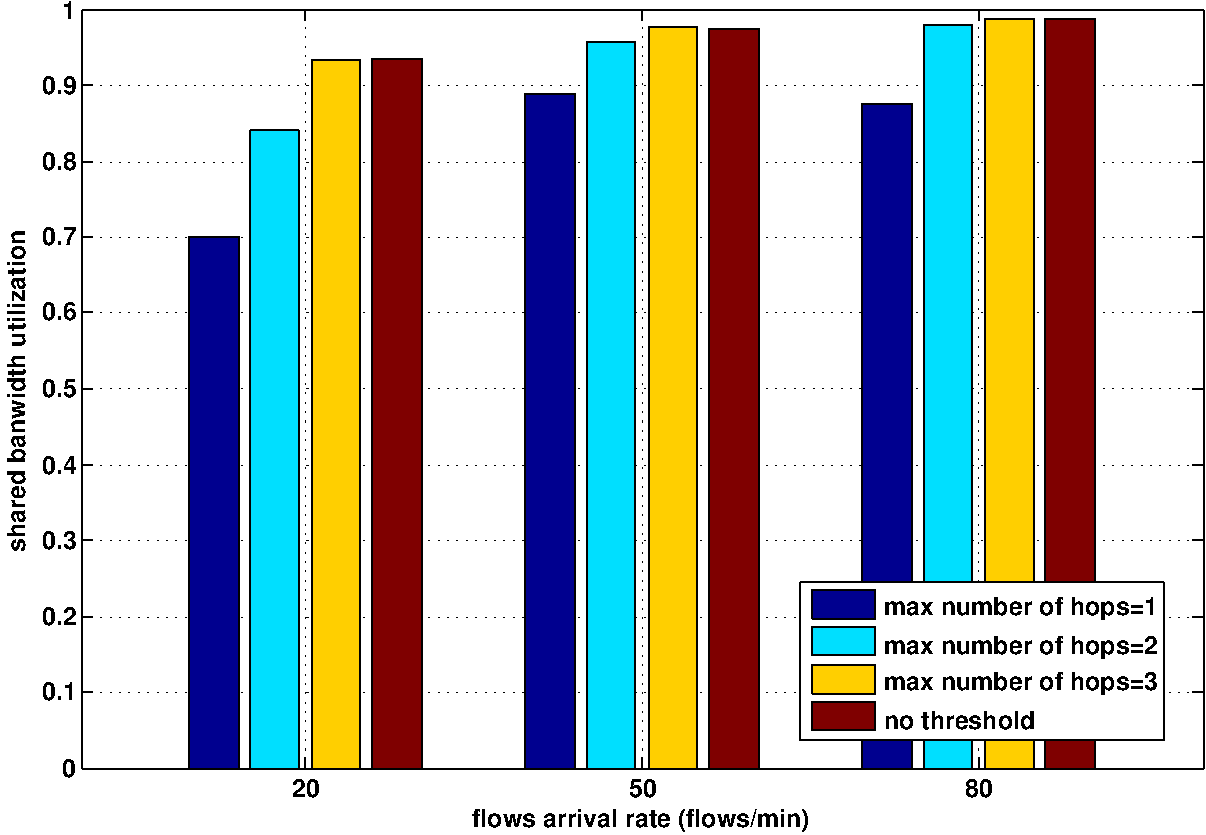
\includegraphics[width=1\linewidth]{results/hops_vs_BW.pdf}
\caption{Shared bandwidth utilization for diverse hop-count threshold values vs. flow arrival rate.}
\label{fig:hop_count}
\end{center}
\end{figure}


\section{Conclusions and Future Work}
\label{sec:conclusion}

In this paper, we quantified the benefits of extending the coverage of any crowd-shared mesh network (e.g., PAWS) by connecting the home routers as a mesh. A crowd-shared WMN can mitigate the fundamental problem of any crowd-shared network, i.e., the presence of a single point of access for each guest user. In a crowd-shared WMN, the path redundancy towards the Internet backhaul can be exploited to achieve better resource utilization, especially during periods of limited Internet access sharing. According to our trace-driven simulations, a crowd-shared WMN can offer much better utilization of the shared bandwidth, providing free Internet access to a larger number of users.

In this paper, SDN and the notion of Virtual Public Networks \cite{EWSDN} constitute the underlying assumptions for the configuration and management of such WMNs by third-party virtual network operators. Although VPuN can facilitate the federation of open wireless home networks and allow their management by a single operator, crowd-shared WMN configuration and management is certainly not a trivial task. For example, decisions for guest user traffic redirections require information about the WMN and access link utilization as well as home user sharing policies. A large WMN may require routing traffic across multiple hops, which, in turn, raises the need for the coordination of flow table updates (e.g., using OpenFlow \cite{OPENFLOW}) in order to avoid packet loss and service disruptions. 

As part of future work, we plan to gain more insights into these problems and investigate solutions by implementing and deploying a SDN control plane in an experimental WMN.  


\section{Acknowledgments}
This work was partially supported by the EPSRC Grant EP/K012703/1. We thank Amr Rizk for his help in modeling the home router on/off periods.

%
% ---- Bibliography ----
%
\begin{thebibliography}{15}

%\bibitem{Airjaldi}
%Airjaldi, http://drupal.airjaldi.com.

%\bibitem{Scotland}
%G. Bernardi, P. Buneman, and M. K. Marina, Tegola tiered mesh network testbed in rural Scotland, ACM MobiCom 2008 Workshop on Wireless Networks and Systems for Developing Regions (WiNS-DR'08), September 2008.

%\bibitem{RFC5281}
%P. Funk and S. Blake-Wilson, Extensible Authentication Protocol Tunneled Transport Layer Security Authenticated Protocol Version 0 (EAP-TTLSv0), RFC 5281, August 2018.

%\bibitem{NOX}
%N. Gude et al., NOX: Towards an operating system for networks, SIGCOM CCR, Vol. 38, No. 3, July 2008, pp. 105-110.

%\bibitem{Hasan}
%S. Hasan et al., Enhancing rural connectivity with software defined networks, ACM DEV, January 2013.

%\bibitem{UN}
%F. La Rue, Report of the Special Rapporteur on the promotion and protection of the right to freedom of opinion and expression, Human Rights Council, UN General Assembly, 16 May 2011, http://goo.gl/MDjS7

%\bibitem{Openflow}
%N. McKeown et al., OpenFlow: Enabling Innovation in Campus Networks, ACM SIGCOMM CCR, Vol. 38, No. 2, pp. 69-74, April 2008.

\bibitem {LCDNet}
A. Sathiaseelan and J. Crowcroft, LCD-Net: lowest cost denominator networking, ACM SIGCOMM CCR Vol. 43, No. 2,  pp. 52-57, April 2013.

\bibitem{EWSDN}
A. Sathiaseelan, C. Rotsos, C.S. Sriram, D. Trossen, P. Papadimitriou, J. Crowcroft, Virtual Public Networks, 2nd IEEE European Workshop on Software Defined Networking (EWSDN), Berlin, October 2013.

\bibitem{PAWS}
A. Sathiaseelan et al., Public Access WiFi Service (PAWS), Digital Economy All Hands Meeting, Aberdeen, October 2012.

\bibitem{BROAD2012}
Broadband lines in the EU, EU document, 2012.

\bibitem{FILD2010}
J. Fildes, UN reveals global disparity in broadband access, BBC, http://www.bbc.co.uk/news/technology-11162656, 2010.

\bibitem{FON}
FON, http://corp.fon.com/

\bibitem{NCC2012} 
Nottingham Citizens Survey, 2012.



%\bibitem{FlowVisor}
%R. Sherwood et al., Can the Production Network Be the Testbed?, USENIX OSDI, Vancouver, October 2010.

%\bibitem{Surana}
%S. Surana et al., Beyond pilots: Keeping rural wireless networks alive, USENIX NSDI, April 2008.




\end{thebibliography}

\end{document}
